% **************************************************************************** %
\section{Python-Code}
\label{app:python}
% **************************************************************************** %


% ---------------------------------------------------------------------------- $
\subsection{Laminare Str\"omung, symbolische Berechnungen}
\label{app:python:Qlaminar}
% ---------------------------------------------------------------------------- $
\lstinputlisting[style=python]{python/Qlaminar.py}


% ---------------------------------------------------------------------------- $
\clearpage
\subsection{Turbulente Str\"omung, symbolische Berechnungen}
\label{app:python:Qturb}
% ---------------------------------------------------------------------------- $
\lstinputlisting[style=python]{python/Qturb.py}


% ---------------------------------------------------------------------------- $
\clearpage
\subsection{Geschwindigkeit in Rohrmitte}
\label{app:python:rohrmitte}
% ---------------------------------------------------------------------------- $
\lstinputlisting[style=python]{python/rohrmitte.py}


% ---------------------------------------------------------------------------- $
\clearpage
\subsection{Str\"omungsprofile im laminaren Fall}
\label{app:python:laminar}
% ---------------------------------------------------------------------------- $
\lstinputlisting[style=python]{python/laminar.py}


% ---------------------------------------------------------------------------- $
\clearpage
\subsection{Str\"omungsprofile im turbulenten Fall}
\label{app:python:turbulent}
% ---------------------------------------------------------------------------- $
\lstinputlisting[style=python]{python/turbulent.py}


% ---------------------------------------------------------------------------- $
\clearpage
\subsection{Fehlerrechnung laminares Str\"omungsprofil}
\label{app:python:errorLaminar}
% ---------------------------------------------------------------------------- $
\lstinputlisting[style=python]{python/errorLaminar.py}

% ---------------------------------------------------------------------------- $
\clearpage
\subsection{Fehlerrechnung turbulentes Str\"omungsprofil}
\label{app:python:errorTurbulent}
% ---------------------------------------------------------------------------- $
\lstinputlisting[style=python]{python/errorTurbulent.py}


% ---------------------------------------------------------------------------- $
\clearpage
\subsection{Umrechnung Messposition zu Position in Messleitung}
\label{app:messposition}
% ---------------------------------------------------------------------------- $

Die  Laserstrahlen   kreuzten  sich   innerhalb  der  Messleitung   bei  einer
Positionsangabe   auf    der   Skala   f\"ur   die    Linse   $L_1$   zwischen
\SI{23}{\milli\meter}   und  \SI{53}{\milli\meter},   was  ein  Intervall  von
\SI{30}{\milli\meter} ergab. Aufgrund des unterschiedlichen Brechungsindex von
Luft Wasser ist dies zu erwarten (siehe Abbildung \ref{fig:lichtbrechung}).

Da   bekannt   ist,   dass   die  Messleitung   einen   Innendurchmesser   von
\SI{40}{\milli\meter}  hat,   wurden  die  Messpositionen  mit   ein  bisschen
Tabellenkalkulation von der Skala auf der Messvorrichtung auf eine Position in
der Messleitung umgerechnet:
\lstinputlisting[%
    basicstyle=\ttfamily\footnotesize\bfseries,
    xleftmargin=0.15\textwidth,
    ]{tables/scales.txt}

Es sei  hier noch  angemerkt, dass dieser  Effekt auf  die Dopplerverschiebung
keinen  Einfluss hat,  weshalb  sie f\"ur  die  Bestimmung des  Schnittwinkels
$\varphi$  in  Abschnitt \ref{subsec:varphi}  (Seite  \pageref{subsec:varphi})
nicht ber\"ucksichtigt wurde.

\vspace{0.5em}
\noindent\adjustbox{valign=t}{\begin{minipage}{0.40\textwidth}
    \captionof{figure}{%
        Verschiebung des  Schnittpunktes der Laserstrahlen in  der Messleitung
        aufgrund der unterschiedlichen Brechungsindizes von Luft und Wasser.
    }
    \label{fig:lichtbrechung}
\end{minipage}}
\adjustbox{valign=t}{\begin{minipage}{0.60\textwidth}
    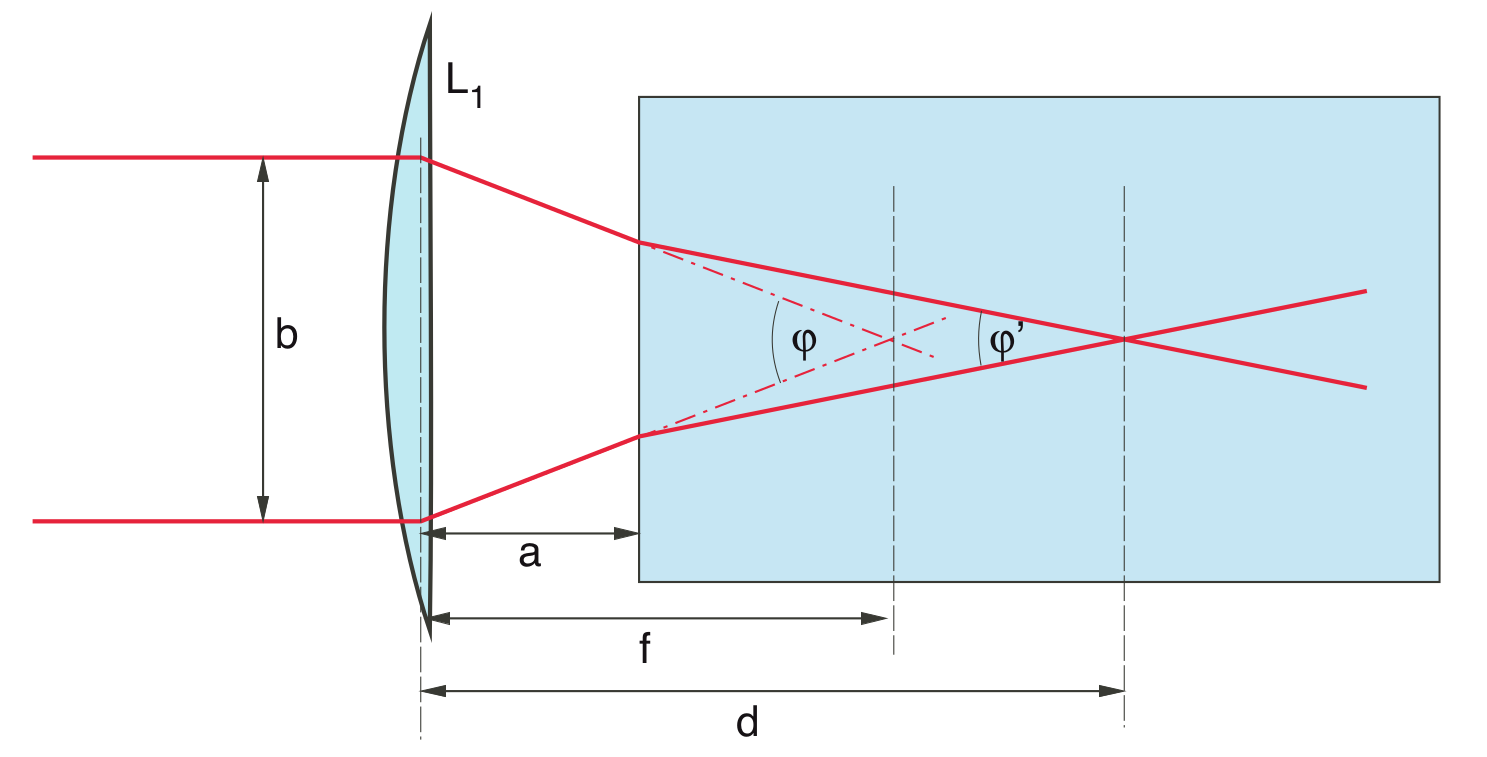
\includegraphics[width=\textwidth]{images/lichtbrechung.png}
\end{minipage}}


% ---------------------------------------------------------------------------- $
\clearpage
\section{Messprotokolle}
\label{app:messprotokolle}
% ---------------------------------------------------------------------------- $
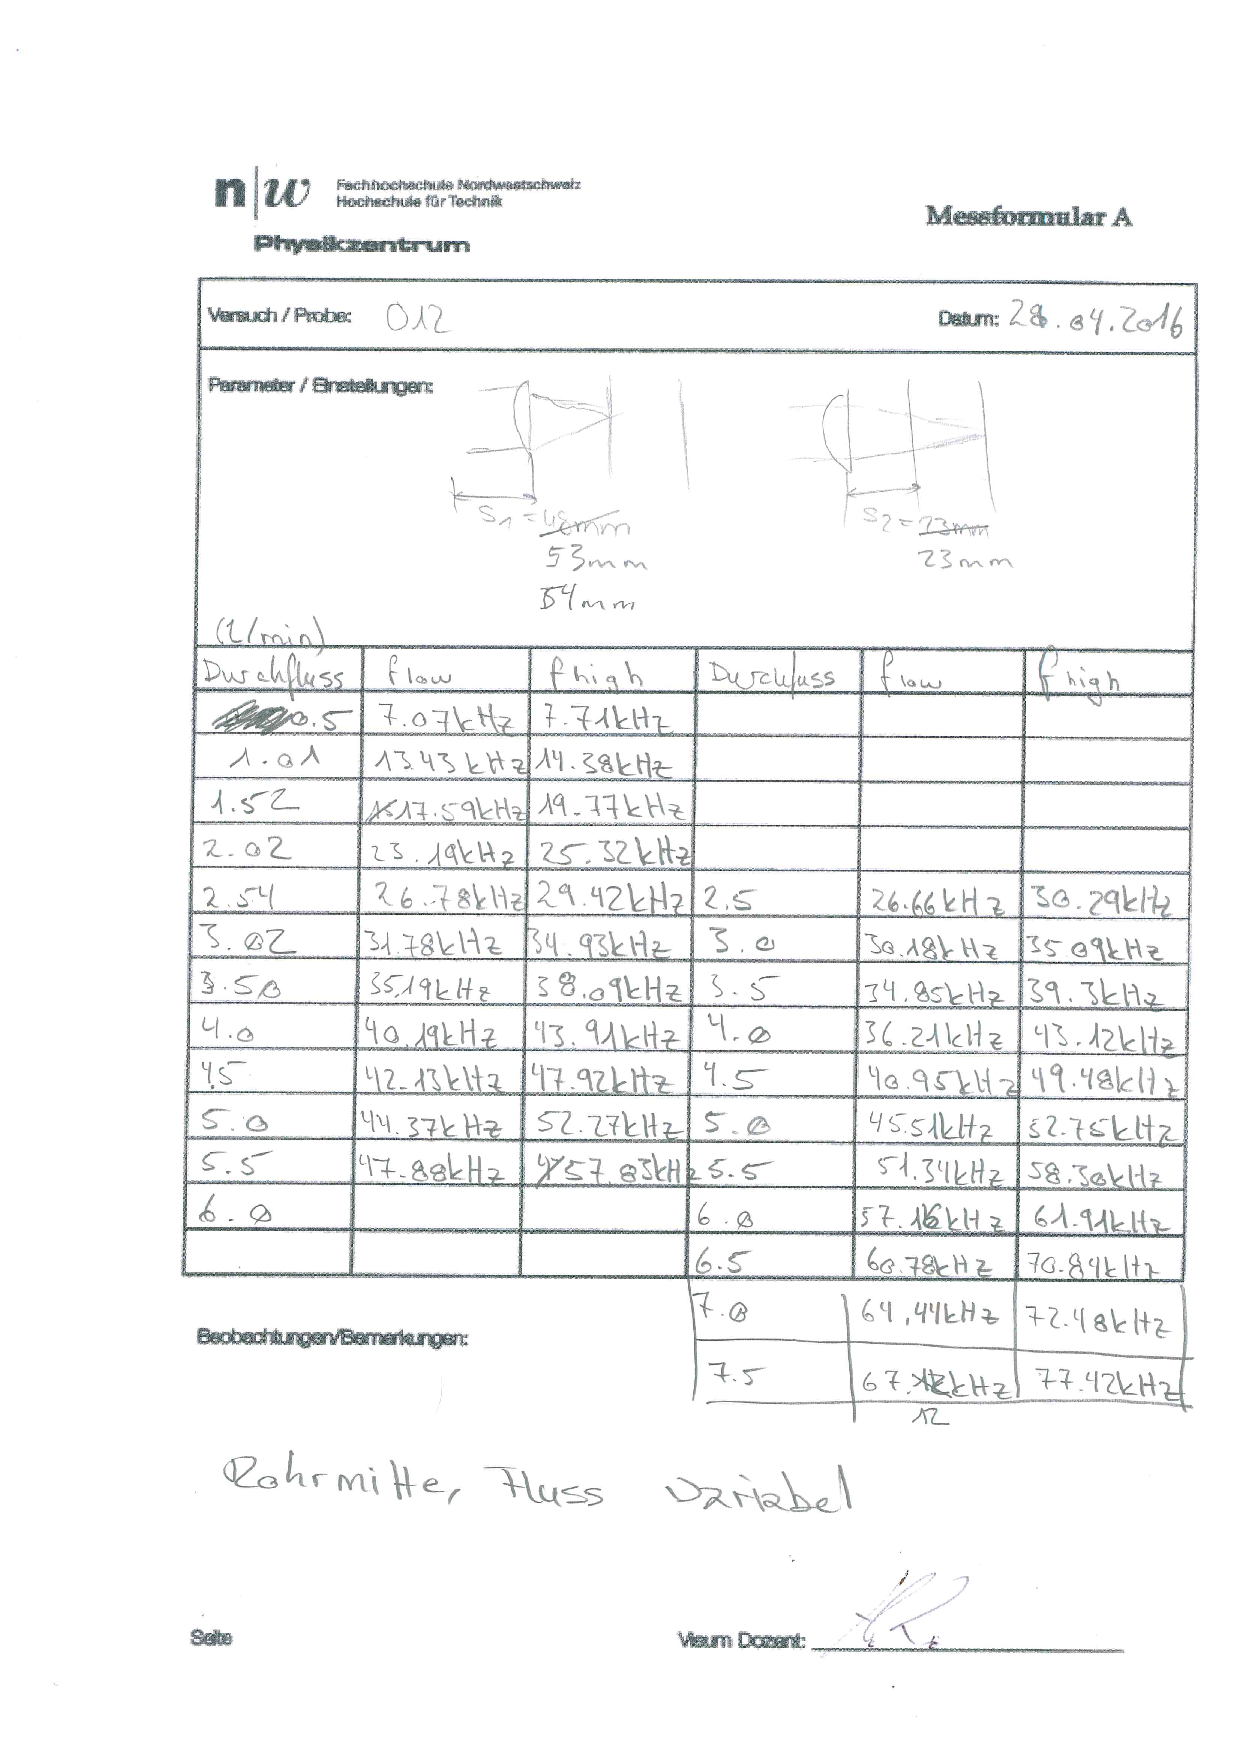
\includepdf[pages=-]{images/messprotokolle.pdf}
